\documentclass{standalone}
\usepackage{tikz}
\usetikzlibrary{patterns, positioning}
\usepackage[sfdefault]{ClearSans} %% option 'sfdefault' activates Clear Sans as the default text font
\usepackage[T1]{fontenc}

\begin{document}
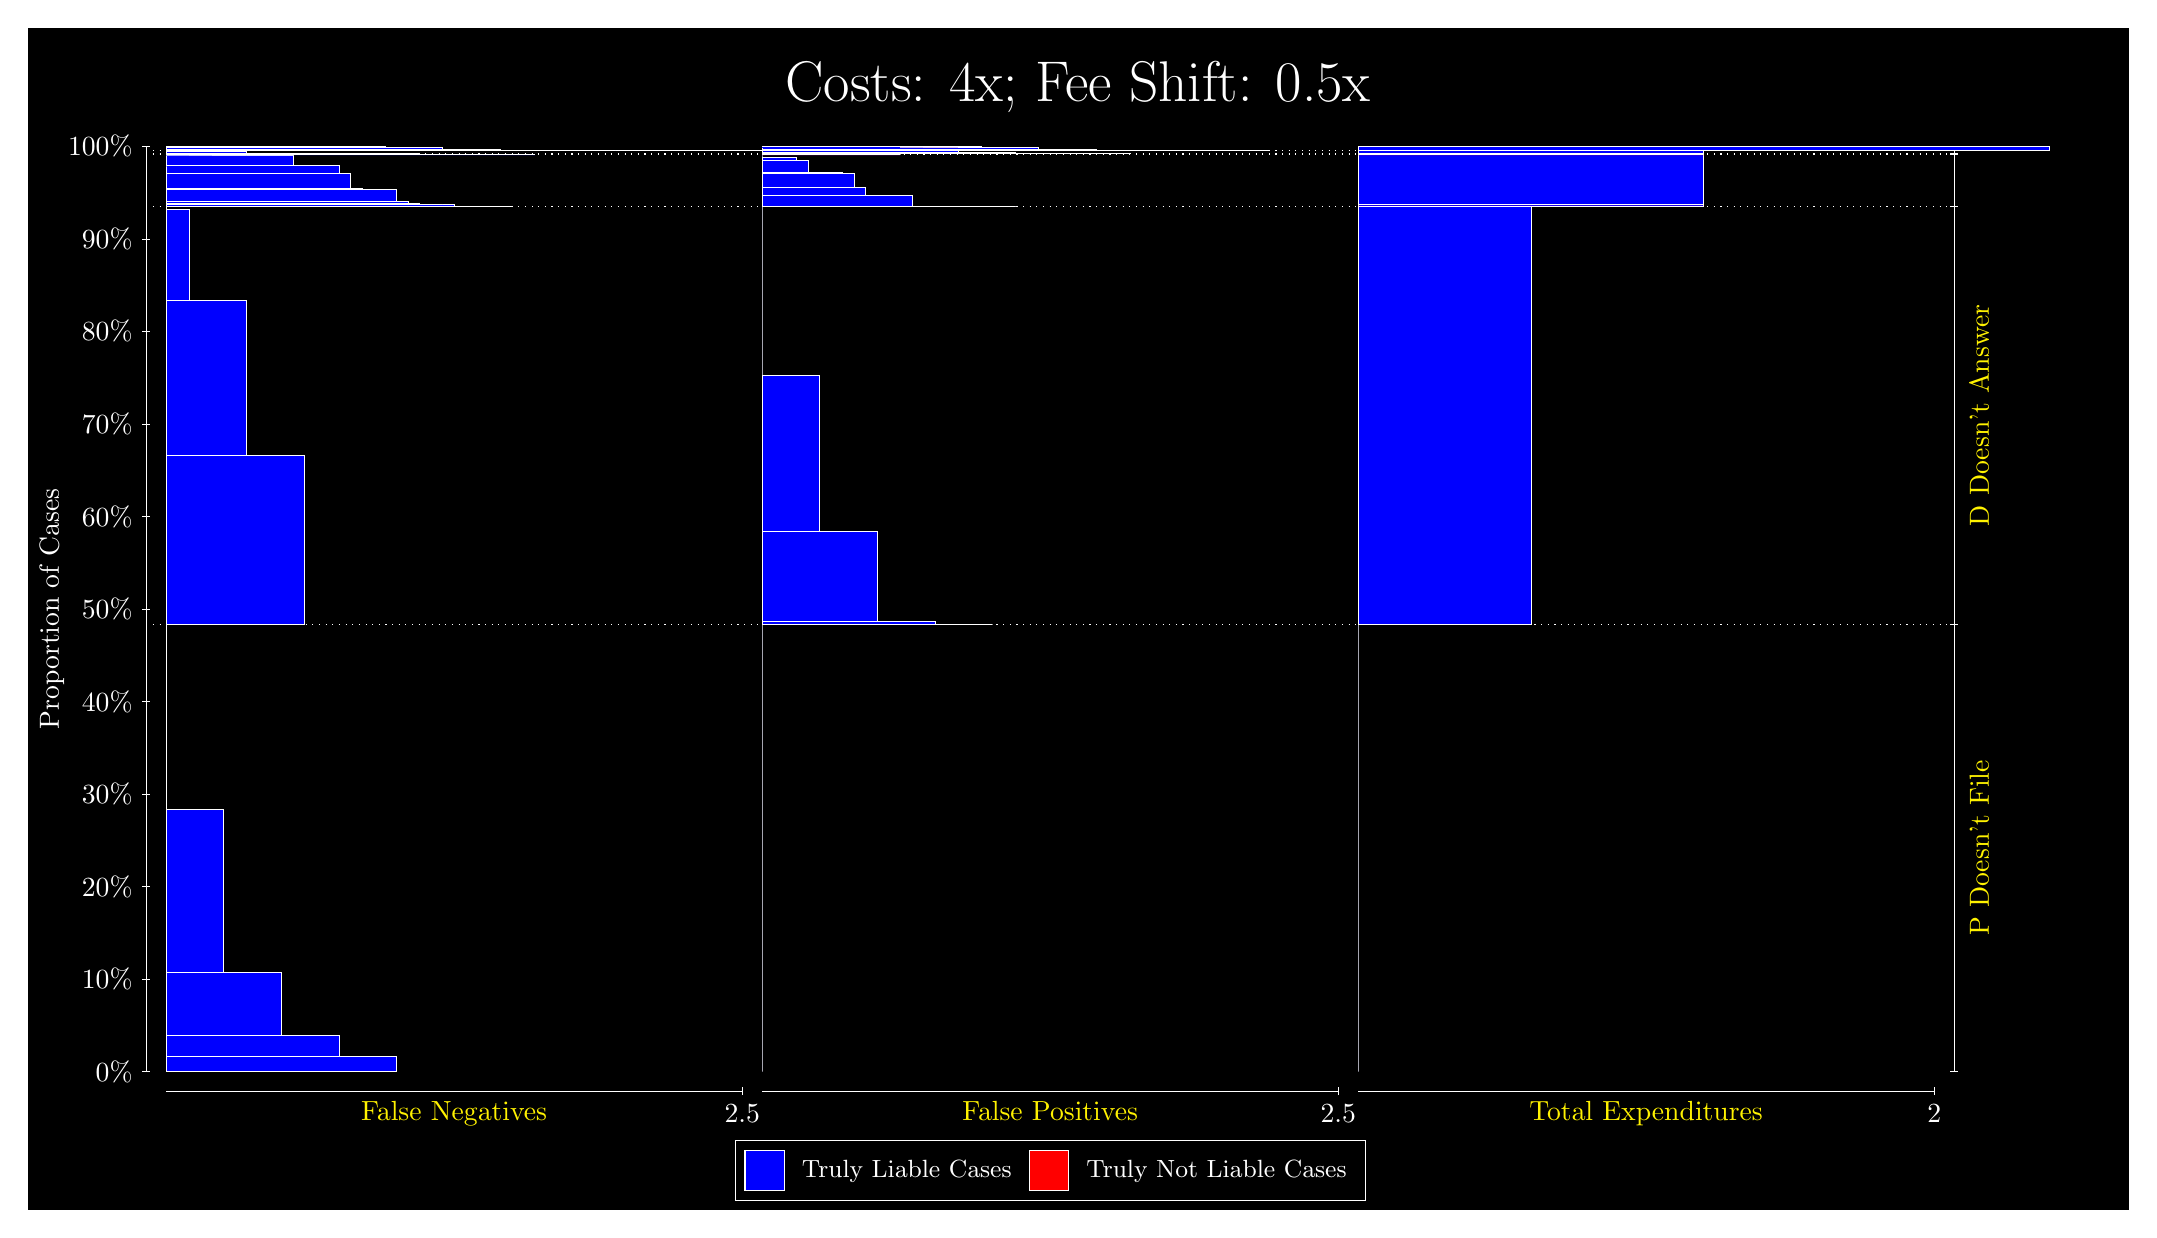
\begin{tikzpicture}
\draw[fill=black] (0,0) rectangle (26.667,15);
\draw[text=white] (0,13.5) rectangle (26.667,15) node[midway] {\huge Costs: 4x; Fee Shift: 0.5x};
\draw[white, very thin] (1.5,1.75) -- (1.5,13.5);
\node[rotate=90, text=white, anchor=center] at (0.3, 7.625) {Proportion of Cases};
\draw[white, very thin] (1.45,1.75) -- (1.55,1.75);
\node[text=white, anchor=east] at (1.45, 1.75) {0\%};
\draw[white, very thin] (1.45,2.925) -- (1.55,2.925);
\node[text=white, anchor=east] at (1.45, 2.925) {10\%};
\draw[white, very thin] (1.45,4.1) -- (1.55,4.1);
\node[text=white, anchor=east] at (1.45, 4.1) {20\%};
\draw[white, very thin] (1.45,5.275) -- (1.55,5.275);
\node[text=white, anchor=east] at (1.45, 5.275) {30\%};
\draw[white, very thin] (1.45,6.45) -- (1.55,6.45);
\node[text=white, anchor=east] at (1.45, 6.45) {40\%};
\draw[white, very thin] (1.45,7.625) -- (1.55,7.625);
\node[text=white, anchor=east] at (1.45, 7.625) {50\%};
\draw[white, very thin] (1.45,8.8) -- (1.55,8.8);
\node[text=white, anchor=east] at (1.45, 8.8) {60\%};
\draw[white, very thin] (1.45,9.975) -- (1.55,9.975);
\node[text=white, anchor=east] at (1.45, 9.975) {70\%};
\draw[white, very thin] (1.45,11.15) -- (1.55,11.15);
\node[text=white, anchor=east] at (1.45, 11.15) {80\%};
\draw[white, very thin] (1.45,12.325) -- (1.55,12.325);
\node[text=white, anchor=east] at (1.45, 12.325) {90\%};
\draw[white, very thin] (1.45,13.5) -- (1.55,13.5);
\node[text=white, anchor=east] at (1.45, 13.5) {100\%};

\draw[white, very thin] (24.457,1.75) -- (24.457,13.5);
\draw[white, very thin] (24.407,1.75) -- (24.507,1.75);
\node[anchor=west] at (24.407, 1.75) {};
\draw[white, very thin] (24.407,7.4286) -- (24.507,7.4286);
\node[anchor=west] at (24.407, 7.4286) {};
\draw[white, very thin] (24.407,12.738) -- (24.507,12.738);
\node[anchor=west] at (24.407, 12.738) {};
\draw[white, very thin] (24.407,13.393) -- (24.507,13.393);
\node[anchor=west] at (24.407, 13.393) {};
\draw[white, very thin] (24.407,13.414) -- (24.507,13.414);
\node[anchor=west] at (24.407, 13.414) {};
\draw[white, very thin] (24.407,13.448) -- (24.507,13.448);
\node[anchor=west] at (24.407, 13.448) {};
\draw[white, very thin] (24.407,13.5) -- (24.507,13.5);
\node[anchor=west] at (24.407, 13.5) {};

\draw[white, very thin, fill=blue] (1.75,1.75) rectangle (4.6775,1.9465);
\draw[white, very thin, fill=blue] (1.75,1.9465) rectangle (3.9457,2.2069);
\draw[white, very thin, fill=blue] (1.75,2.2069) rectangle (3.2138,3.0119);
\draw[white, very thin, fill=blue] (1.75,3.0119) rectangle (2.4819,5.0814);
\draw[white, very thin, fill=red] (1.75,5.0814) rectangle (1.75,5.0814);
\draw[white, very thin, fill=blue] (1.75,5.0814) rectangle (1.75,7.4286);
\draw[white, very thin, fill=blue] (1.75,7.4286) rectangle (3.5065,9.5726);
\draw[white, very thin, fill=blue] (1.75,9.5726) rectangle (2.7746,11.551);
\draw[white, very thin, fill=blue] (1.75,11.551) rectangle (2.0428,12.698);
\draw[white, very thin, fill=red] (1.75,12.698) rectangle (1.75,12.698);
\draw[white, very thin, fill=blue] (1.75,12.698) rectangle (1.75,12.738);
\draw[white, very thin, fill=blue] (1.75,12.738) rectangle (6.1413,12.738);
\draw[white, very thin, fill=blue] (1.75,12.738) rectangle (5.8486,12.738);
\draw[white, very thin, fill=blue] (1.75,12.738) rectangle (5.5558,12.739);
\draw[white, very thin, fill=blue] (1.75,12.739) rectangle (5.4094,12.764);
\draw[white, very thin, fill=blue] (1.75,12.764) rectangle (5.2631,12.764);
\draw[white, very thin, fill=blue] (1.75,12.764) rectangle (5.1167,12.767);
\draw[white, very thin, fill=blue] (1.75,12.767) rectangle (4.9703,12.774);
\draw[white, very thin, fill=blue] (1.75,12.774) rectangle (4.8239,12.804);
\draw[white, very thin, fill=blue] (1.75,12.804) rectangle (4.6775,12.955);
\draw[white, very thin, fill=blue] (1.75,12.955) rectangle (4.5312,12.957);
\draw[white, very thin, fill=blue] (1.75,12.957) rectangle (4.3848,12.959);
\draw[white, very thin, fill=blue] (1.75,12.959) rectangle (4.2384,12.973);
\draw[white, very thin, fill=blue] (1.75,12.973) rectangle (4.092,13.152);
\draw[white, very thin, fill=blue] (1.75,13.152) rectangle (3.9457,13.254);
\draw[white, very thin, fill=blue] (1.75,13.254) rectangle (3.7993,13.254);
\draw[white, very thin, fill=blue] (1.75,13.254) rectangle (3.6529,13.254);
\draw[white, very thin, fill=blue] (1.75,13.254) rectangle (3.5065,13.257);
\draw[white, very thin, fill=blue] (1.75,13.257) rectangle (3.3602,13.39);
\draw[white, very thin, fill=blue] (1.75,13.39) rectangle (3.2138,13.391);
\draw[white, very thin, fill=blue] (1.75,13.391) rectangle (3.0674,13.391);
\draw[white, very thin, fill=blue] (1.75,13.391) rectangle (2.921,13.391);
\draw[white, very thin, fill=blue] (1.75,13.391) rectangle (2.7746,13.391);
\draw[white, very thin, fill=blue] (1.75,13.391) rectangle (2.6283,13.393);
\draw[white, very thin, fill=blue] (1.75,13.393) rectangle (2.3355,13.393);
\draw[white, very thin, fill=blue] (1.75,13.393) rectangle (2.0428,13.393);
\draw[white, very thin, fill=red] (1.75,13.393) rectangle (1.75,13.393);
\draw[white, very thin, fill=blue] (1.75,13.393) rectangle (6.4341,13.393);
\draw[white, very thin, fill=blue] (1.75,13.393) rectangle (5.7022,13.398);
\draw[white, very thin, fill=blue] (1.75,13.398) rectangle (4.9703,13.409);
\draw[white, very thin, fill=blue] (1.75,13.409) rectangle (4.2384,13.414);
\draw[white, very thin, fill=blue] (1.75,13.414) rectangle (3.5065,13.414);
\draw[white, very thin, fill=red] (1.75,13.414) rectangle (1.75,13.414);
\draw[white, very thin, fill=blue] (1.75,13.414) rectangle (3.5065,13.414);
\draw[white, very thin, fill=blue] (1.75,13.414) rectangle (2.7746,13.433);
\draw[white, very thin, fill=blue] (1.75,13.433) rectangle (2.0428,13.448);
\draw[white, very thin, fill=red] (1.75,13.448) rectangle (1.75,13.448);
\draw[white, very thin, fill=blue] (1.75,13.448) rectangle (1.75,13.448);
\draw[white, very thin, fill=blue] (1.75,13.448) rectangle (9.9471,13.448);
\draw[white, very thin, fill=blue] (1.75,13.448) rectangle (9.2152,13.448);
\draw[white, very thin, fill=blue] (1.75,13.448) rectangle (8.4834,13.449);
\draw[white, very thin, fill=blue] (1.75,13.449) rectangle (7.7515,13.452);
\draw[white, very thin, fill=blue] (1.75,13.452) rectangle (7.4587,13.452);
\draw[white, very thin, fill=blue] (1.75,13.452) rectangle (7.0196,13.452);
\draw[white, very thin, fill=blue] (1.75,13.452) rectangle (6.7268,13.452);
\draw[white, very thin, fill=blue] (1.75,13.452) rectangle (6.2877,13.452);
\draw[white, very thin, fill=blue] (1.75,13.452) rectangle (5.9949,13.462);
\draw[white, very thin, fill=blue] (1.75,13.462) rectangle (5.2631,13.487);
\draw[white, very thin, fill=blue] (1.75,13.487) rectangle (4.5312,13.499);
\draw[white, very thin, fill=blue] (1.75,13.499) rectangle (3.7993,13.5);
\draw[white, very thin, fill=blue] (1.75,13.5) rectangle (3.0674,13.5);
\draw[white, very thin, fill=blue] (1.75,13.5) rectangle (2.3355,13.5);
\draw[white, very thin, fill=red] (1.75,13.5) rectangle (1.75,13.5);
\draw[white, very thin, fill=red] (9.3189,1.75) rectangle (9.3189,1.75);
\draw[white, very thin, fill=blue] (9.3189,1.75) rectangle (9.3189,7.4286);
\draw[white, very thin, fill=red] (9.3189,7.4286) rectangle (12.246,7.4286);
\draw[white, very thin, fill=blue] (9.3189,7.4286) rectangle (12.246,7.4286);
\draw[white, very thin, fill=blue] (9.3189,7.4286) rectangle (11.515,7.4683);
\draw[white, very thin, fill=blue] (9.3189,7.4683) rectangle (10.783,8.6152);
\draw[white, very thin, fill=blue] (9.3189,8.6152) rectangle (10.051,10.594);
\draw[white, very thin, fill=blue] (9.3189,10.594) rectangle (9.3189,12.738);
\draw[white, very thin, fill=red] (9.3189,12.738) rectangle (12.539,12.738);
\draw[white, very thin, fill=blue] (9.3189,12.738) rectangle (12.539,12.738);
\draw[white, very thin, fill=red] (9.3189,12.738) rectangle (12.246,12.738);
\draw[white, very thin, fill=blue] (9.3189,12.738) rectangle (12.246,12.738);
\draw[white, very thin, fill=red] (9.3189,12.738) rectangle (11.954,12.738);
\draw[white, very thin, fill=blue] (9.3189,12.738) rectangle (11.954,12.74);
\draw[white, very thin, fill=blue] (9.3189,12.74) rectangle (11.807,12.74);
\draw[white, very thin, fill=red] (9.3189,12.74) rectangle (11.661,12.74);
\draw[white, very thin, fill=blue] (9.3189,12.74) rectangle (11.661,12.74);
\draw[white, very thin, fill=blue] (9.3189,12.74) rectangle (11.515,12.74);
\draw[white, very thin, fill=red] (9.3189,12.74) rectangle (11.368,12.74);
\draw[white, very thin, fill=blue] (9.3189,12.74) rectangle (11.368,12.741);
\draw[white, very thin, fill=blue] (9.3189,12.741) rectangle (11.222,12.874);
\draw[white, very thin, fill=blue] (9.3189,12.874) rectangle (11.075,12.876);
\draw[white, very thin, fill=blue] (9.3189,12.876) rectangle (10.929,12.876);
\draw[white, very thin, fill=blue] (9.3189,12.876) rectangle (10.783,12.876);
\draw[white, very thin, fill=blue] (9.3189,12.876) rectangle (10.636,12.978);
\draw[white, very thin, fill=blue] (9.3189,12.978) rectangle (10.49,13.158);
\draw[white, very thin, fill=blue] (9.3189,13.158) rectangle (10.344,13.171);
\draw[white, very thin, fill=blue] (9.3189,13.171) rectangle (10.197,13.174);
\draw[white, very thin, fill=blue] (9.3189,13.174) rectangle (10.051,13.175);
\draw[white, very thin, fill=blue] (9.3189,13.175) rectangle (9.9044,13.326);
\draw[white, very thin, fill=blue] (9.3189,13.326) rectangle (9.758,13.357);
\draw[white, very thin, fill=blue] (9.3189,13.357) rectangle (9.6116,13.364);
\draw[white, very thin, fill=blue] (9.3189,13.364) rectangle (9.4652,13.366);
\draw[white, very thin, fill=blue] (9.3189,13.366) rectangle (9.3189,13.393);
\draw[white, very thin, fill=red] (9.3189,13.393) rectangle (11.075,13.393);
\draw[white, very thin, fill=blue] (9.3189,13.393) rectangle (11.075,13.393);
\draw[white, very thin, fill=blue] (9.3189,13.393) rectangle (10.344,13.397);
\draw[white, very thin, fill=blue] (9.3189,13.397) rectangle (9.6116,13.408);
\draw[white, very thin, fill=blue] (9.3189,13.408) rectangle (9.3189,13.414);
\draw[white, very thin, fill=red] (9.3189,13.414) rectangle (14.003,13.414);
\draw[white, very thin, fill=blue] (9.3189,13.414) rectangle (14.003,13.414);
\draw[white, very thin, fill=blue] (9.3189,13.414) rectangle (13.271,13.414);
\draw[white, very thin, fill=blue] (9.3189,13.414) rectangle (12.539,13.429);
\draw[white, very thin, fill=blue] (9.3189,13.429) rectangle (11.807,13.448);
\draw[white, very thin, fill=blue] (9.3189,13.448) rectangle (11.075,13.448);
\draw[white, very thin, fill=red] (9.3189,13.448) rectangle (15.759,13.448);
\draw[white, very thin, fill=blue] (9.3189,13.448) rectangle (15.759,13.448);
\draw[white, very thin, fill=blue] (9.3189,13.448) rectangle (15.028,13.448);
\draw[white, very thin, fill=red] (9.3189,13.448) rectangle (15.028,13.448);
\draw[white, very thin, fill=blue] (9.3189,13.448) rectangle (15.028,13.448);
\draw[white, very thin, fill=blue] (9.3189,13.448) rectangle (14.296,13.449);
\draw[white, very thin, fill=red] (9.3189,13.449) rectangle (14.296,13.449);
\draw[white, very thin, fill=blue] (9.3189,13.449) rectangle (14.296,13.449);
\draw[white, very thin, fill=blue] (9.3189,13.449) rectangle (13.564,13.453);
\draw[white, very thin, fill=red] (9.3189,13.453) rectangle (13.564,13.453);
\draw[white, very thin, fill=blue] (9.3189,13.453) rectangle (13.564,13.461);
\draw[white, very thin, fill=blue] (9.3189,13.461) rectangle (12.832,13.461);
\draw[white, very thin, fill=blue] (9.3189,13.461) rectangle (12.832,13.487);
\draw[white, very thin, fill=blue] (9.3189,13.487) rectangle (12.1,13.496);
\draw[white, very thin, fill=red] (9.3189,13.496) rectangle (11.807,13.496);
\draw[white, very thin, fill=blue] (9.3189,13.496) rectangle (11.807,13.496);
\draw[white, very thin, fill=blue] (9.3189,13.496) rectangle (11.368,13.496);
\draw[white, very thin, fill=red] (9.3189,13.496) rectangle (11.075,13.496);
\draw[white, very thin, fill=blue] (9.3189,13.496) rectangle (11.075,13.497);
\draw[white, very thin, fill=blue] (9.3189,13.497) rectangle (10.636,13.497);
\draw[white, very thin, fill=blue] (9.3189,13.497) rectangle (10.344,13.499);
\draw[white, very thin, fill=blue] (9.3189,13.499) rectangle (9.6116,13.5);
\draw[white, very thin, fill=blue] (9.3189,13.5) rectangle (9.3189,13.5);
\draw[white, very thin, fill=red] (16.888,1.75) rectangle (16.888,1.75);
\draw[white, very thin, fill=blue] (16.888,1.75) rectangle (16.888,7.4286);
\draw[white, very thin, fill=red] (16.888,7.4286) rectangle (19.083,7.4286);
\draw[white, very thin, fill=blue] (16.888,7.4286) rectangle (19.083,12.738);
\draw[white, very thin, fill=red] (16.888,12.738) rectangle (21.279,12.738);
\draw[white, very thin, fill=blue] (16.888,12.738) rectangle (21.279,12.761);
\draw[white, very thin, fill=red] (16.888,12.761) rectangle (21.279,12.761);
\draw[white, very thin, fill=blue] (16.888,12.761) rectangle (21.279,13.393);
\draw[white, very thin, fill=red] (16.888,13.393) rectangle (21.279,13.393);
\draw[white, very thin, fill=blue] (16.888,13.393) rectangle (21.279,13.414);
\draw[white, very thin, fill=red] (16.888,13.414) rectangle (21.279,13.414);
\draw[white, very thin, fill=blue] (16.888,13.414) rectangle (21.279,13.448);
\draw[white, very thin, fill=red] (16.888,13.448) rectangle (25.67,13.448);
\draw[white, very thin, fill=blue] (16.888,13.448) rectangle (25.67,13.453);
\draw[white, very thin, fill=red] (16.888,13.453) rectangle (25.67,13.453);
\draw[white, very thin, fill=blue] (16.888,13.453) rectangle (25.67,13.5);
\draw[white, dotted] (1.5,7.4286) -- (24.457,7.4286);
\draw[white, dotted] (1.5,12.738) -- (24.457,12.738);
\draw[white, dotted] (1.5,13.393) -- (24.457,13.393);
\draw[white, dotted] (1.5,13.414) -- (24.457,13.414);
\draw[white, dotted] (1.5,13.448) -- (24.457,13.448);
\draw[white, very thin] (1.75,1.5) -- (9.0689,1.5);
\node[text=yellow, anchor=north] at (5.4094, 1.5) {False Negatives};
\draw[white, very thin] (9.0689,1.45) -- (9.0689,1.55);
\node[text=white, anchor=north] at (9.0689, 1.45) {2.5};

\draw[white, very thin] (9.3189,1.5) -- (16.638,1.5);
\node[text=yellow, anchor=north] at (12.978, 1.5) {False Positives};
\draw[white, very thin] (16.638,1.45) -- (16.638,1.55);
\node[text=white, anchor=north] at (16.638, 1.45) {2.5};

\draw[white, very thin] (16.888,1.5) -- (24.207,1.5);
\node[text=yellow, anchor=north] at (20.547, 1.5) {Total Expenditures};
\draw[white, very thin] (24.207,1.45) -- (24.207,1.55);
\node[text=white, anchor=north] at (24.207, 1.45) {2};

\node[text=yellow, centered, rotate=90] at (24.777, 4.5893) {P Doesn't File};
\node[text=yellow, centered, rotate=90] at (24.777, 10.083) {D Doesn't Answer};





\draw (12.978300999999998,1.5) node[draw=none] (baseCoordinate) {};
\begin{scope}[align=center]
        \matrix[scale=0.5, draw=white, below=0.5cm of baseCoordinate, nodes={draw}, column sep=0.1cm]{
            \node[rectangle, draw, minimum width=0.5cm, minimum height=0.5cm, fill=blue] {}; &
            \node[draw=none, font=\small, text=white] (B) {Truly Liable Cases}; &
            \node[rectangle, draw, minimum width=0.5cm, minimum height=0.5cm, fill=red] {}; &
            \node[draw=none, font=\small, text=white] (B) {Truly Not Liable Cases}; \\
            };
\end{scope}

\end{tikzpicture}
\end{document}